In triangle $ABC$, $BC = 23$, $CA = 27$, and $AB = 30$.  Points $V$ and $W$ are on $\overline{AC}$ with $V$ on $\overline{AW}$, points $X$ and $Y$ are on $\overline{BC}$ with $X$ on $\overline{CY}$, and points $Z$ and $U$ are on $\overline{AB}$ with $Z$ on $\overline{BU}$.  In addition, the points are positioned so that $\overline{UV} \parallel \overline{BC}$, $\overline{WX} \parallel \overline{AB}$, and $\overline{YZ} \parallel \overline{CA}$.  Right angle folds are then made along $\overline{UV}$, $\overline{WX}$, and $\overline{YZ}$.  The resulting figure is placed on a level floor to make a table with triangular legs.  Let $h$ be the maximum possible height of a table constructed from triangle $ABC$ whose top is parallel to the floor.  Then $h$ can be written in the form $\tfrac{k \sqrt{m}}{n}$, where $k$ and $n$ are relatively prime positive integers and $m$ is a positive integer that is not divisible by the square of any prime.  Find $k + m + n$.

\begin{center}
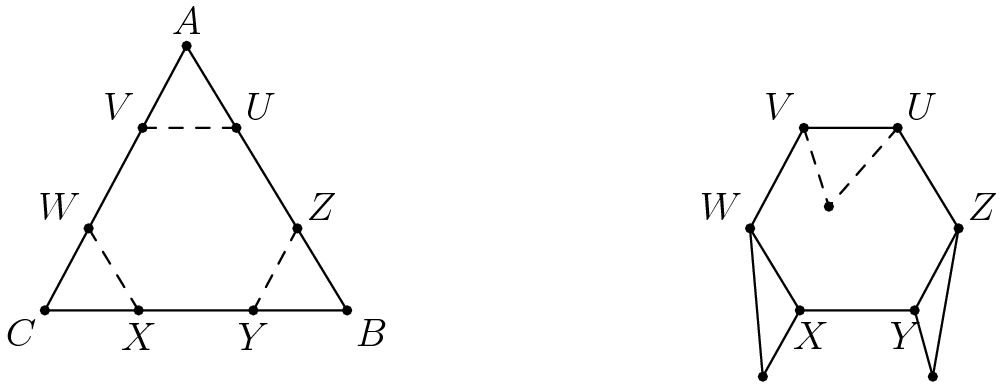
\includegraphics[width = 100.4mm]{img/fig0.png}
\end{center}